% --------------------------------------------------------------------------
% Template for DCASE 2018 paper; to be used with:
%          dcase2018.sty  - DCASE 2018 LaTeX style file, and
%          IEEEbib.bst - IEEE bibliography style file.
% Adapted from spconf.sty and waspaa15.sty
% --------------------------------------------------------------------------

\documentclass{article}
\usepackage{dcase2018,amsmath,graphicx,url,times,booktabs, tabularx}
\usepackage{bbm}

\usepackage{color}
\newcommand{\ml}[1]{\textcolor{blue}{ Mathieu : #1}}
% Example definitions.
% --------------------
\def\defeqn{\stackrel{\triangle}{=}}
\newcommand{\symvec}[1]{{\mbox{\boldmath $#1$}}}
\newcommand{\symmat}[1]{{\mbox{\boldmath $#1$}}}

% Title.
% --------------------
\title{Towards perceptual soundscape characterization using event detection algorithms}

\name{F\'elix Gontier$^{1}$,
Pierre Aumond$^{2, 3}$,
Mathieu Lagrange$^{1}$,
       }
 \secondlinename{
       Catherine Lavandier$^{2}$,
       Jean-Francois Petiot$^{1}$
       }
       % fixed *.sty to allow names on multiple lines
 \address{$^1$ LS2N, UMR 6004, Ecole Centrale de Nantes, CNRS, 44322 Nantes, France, \{felix.gontier\}@ls2n.fr\\
         $^2$ ETIS, UMR 8051, Universit\'e Paris Seine, Universit\'e de Cergy-Pontoise, ENSEA, CNRS, France\\ %\\ 95000 Cergy-Pontoise
         $^3$ IFSTTAR, CEREMA, UMRAE, F-44344 Bouguenais, France\\
  }

\begin{document}



\ninept
\maketitle

\begin{sloppy}

\begin{abstract}
Assessing properties about specific sound sources is important to  characterize better the perception of urban sound environments. In order to produce perceptually motivated noise maps, we argue that it is possible to consider the data produced by acoustic sensor networks to gather information about sources of interest and predict their perceptual attributes.

To validate this important assumption, this paper reports on a perceptual test on simulated sound scenes for which both perceptual and acoustic source properties are known. Results show that it is indeed feasible to predict perceptual source-specific quantities of interest from recordings, leading to the introduction of two predictors of perceptual judgments from acoustic data. The use of those predictors in the new task of automatic soundscape characterization is finally discussed.

\end{abstract}

\begin{keywords}
  Soundscape, urban acoustic monitoring, event detection
\end{keywords}

\section{Introduction}
\label{sec:intro}

The ongoing urbanization process has led to an increase in sound quality concerns. In urban areas the noise has been linked to several health issues including sleep-related troubles as well as heart disease rates, and is a major cause for city dwellers' annoyance in certain areas. In this context, the 2002/49/CE European directive~\cite{ec2002} requires that large cities maintain noise maps to facilitate the development of noise reducing plans. These noise maps are mainly based on predictive maps generated using propagation and emission acoustic models. The studies are also 1) often limited to traffic and other transportation sources, and 2) no fusions of simulations with physical measurements are used. Furthermore, the models depend on data that may be at times or in certain locations unavailable or incomplete. The advent of the internet of things (IoT) presents an opportunity for the development of large, scalable networks of acoustic sensors~\cite{mydlarz2017, gontier2017}. The "characterization of urban sound environments" (CENSE) project~\cite{picault2017} aims at implementing such a network to produce perceptually motivated noise maps.


The ISO 12913-1~\cite{iso2014} standard gives the following definition of soundscape: "the acoustic environment as perceived and understood and/or experienced by people and/or society, in context". The assessment of subjective descriptors~\cite{berglund2006, brown2011, aletta2016} such as the liveliness or calmness is thus necessary to evaluate the quality of urban scenes. The relevant attributes describing the appreciation of soundscapes can be mapped in perceptual spaces~\cite{axelsson2010, cain2013}. The set of considered attributes is reduced to a few dimensions which are used as a basis for perceptual experiments. Specifically, the dimension of pleasantness is increasingly associated with soundscape quality in recent works~\cite{decoensel2006, delaitre2014, ricciardi2014, aumond2017}. Soundscape perception is highly dependent on the composition of the scene~\cite{lavandier2006, nilsson2006}. Indeed, each sound source yields a different perceptual response. For example, soundscape pleasantness is likely to be improved by birdsongs and deteriorated by mechanical noises.

Acoustic monitoring applications typically rely on the measurement of energetic (sound levels, eg. $L_{Aeq}$) and psychoacoustic (eg. Zwicker's loudness $N$) indicators. These global quantities describe the overall activity, with percentile values linked to event or background assessment. However they do not differentiate sound sources and are thus not sufficient to a perceptual characterization of soundscapes. Additional information about the taxonomic classification of active sources and their distribution in time is needed. Several sets of relevant indicators have been studied~\cite{can2008, can2016, brocolini2013} to better account for the specificities of each scene and their source composition.

The use of large-scale sensor networks yields a problematic for the extraction of content-related quantities of interest from important amounts of data. Despite a growing interest in the community, machine learning models - to the best of our knowledge - were not yet specifically targeted to the prediction of source-specific perceptual parameters in complex urban environments. Most event detection applications focus on obtaining a precise annotation of source activity, within usual ranges of tens of milliseconds. The estimation of sound levels involves entirely different models through source separation and regression \cite{gloaguen2016} and longer time scales.

We believe that the use of machine listening techniques could greatly benefit the automatic assessment of urban soundscape quality using sensor networks. The aim of this paper is to 1) bring some context of soundscape characterization, and 2) report on a perceptual experiment performed in order to study which features shall be brought by automatic event detection systems in order to gather relevant information for the task of characterize perceptual attributes of the soundscape.


\section{Soundscape Characterization}
\label{sec:char}

Urban soundscape monitoring has only scarcely been studied by the machine listening community\cite{bello2018}. This work aims at contributing to this task by focusing on pleasantness as it is the most recurrent descriptor of urban soundscape quality, though similar studies could be led for other notions such as liveliness.

Several perceptual experiments on the urban soundscape quality have indeed proposed a model of pleasantness from other perceptual parameters~\cite{nilsson2007, axelsson2010, aumond2017, ricciardi2014}. In all cases, a good approximation of pleasantness can be obtained by linear combination of both overall and source-specific parameters evaluated on discrete scales. Global parameters consider the sound scene in its entirety for which the overall loudness is commonly used. The parameters used for the assessment of source-wise contributions include 1) the sound level where each source is considered separately, 2) the emergence or dominance relating to the influence of the source in the global mix, or 3) the time of presence, that is the ratio of time where the source $s$ is heard in a given scene. The notion of time of presence is particularly interesting as it hints at the possibility of automatic prediction through event detection systems. The corresponding model is:
\begin{equation}
P = aL + \sum_s b_sT_{s,p} + c
\end{equation}
where $P$ is the scene's pleasantness, $L$ is the perceived overall level and $T_{s,p}$ is the perceived time of presence for source $s$. These parameters are evaluated on discrete scales through perceptual tests. The coefficients $a$, $b_s$ and $c$ are usually found via multiple linear regression and thus differ in each study.
Furthermore, three principal source categories are usually identified: mechanical, human and nature. Mechanical sounds are mainly composed of traffic and are mostly found to have a negative impact on soundscape pleasantness, whereas nature sources such as bird activity or water sounds have a positive influence and human sounds (voices) can yield mixed effects.


\begin{figure}[t]
  \centering
  \centerline{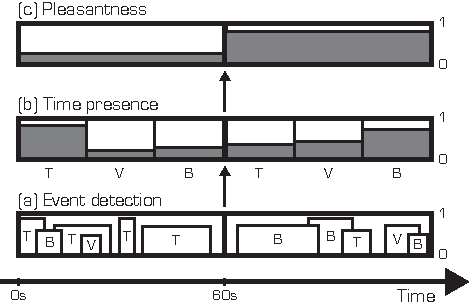
\includegraphics[width=0.8\columnwidth]{block.pdf}}
  \caption{The three suggested levels of metrics to predict soundscape pleasantness. (a) Traffic (T), voice (V) and bird (B) events are detected and their sound level roughly estimated. (b) The perceptual time of presence for each source is computed on one-minute frames, resulting in a pleasantness value (c).}
  \label{fig:block}
\end{figure}

Assuming this perceptual model, the prediction of pleasantness can be assimilated as that of perceived times of presence of sources. Three levels of metrics are thus identified for this task. First, the physical level Figure~\ref{fig:block}(a) is evaluated on the presence and emergence of the three identified sound sources: traffic (T), voice (V) and birds (B). The precision of event onset and sound level estimations needed to achieve the task is further studied in this paper. The second level Figure~\ref{fig:block}(b) is the perceived time of presence for each source in the whole scene represented as a scalar in the 0-1 range. The third level Figure~\ref{fig:block}(c) is the estimate of pleasantness over the scene, also represented as a 0-1 scalar. Both the perceptual levels of metrics are only relevant on longer time scales, about one minute being a usual value in existing experiments.

The transition model between the perceived time of presence per source and pleasantness has already been proposed. However no previous work exists that uses detection models for the estimation of source-specific subjective parameters. The feasibility of assessing source perception from the postulated metrics at the physical level shall be verified as a first step prior to building the full estimation model.

\section{From physical to perceptual time of presence of sources}
\label{sec:val}

We thus conduct a perceptual experiment to validate this key step of the estimation procedure. We wish to study the relation between extracted source-dependent physical indicators to their perceptual equivalents, then validate the relevance of the first level of metrics introduced in the previous section.

\subsection{Perceptual Test}

For this test, a set of sound scenes recorded in the 13th district of Paris as part of the GRAFIC project~\cite{aumond2017} is used as reference. Some artificial scenes with equivalent event sequencing are also used for which the acoustic properties of each source of the scene can be computed precisely.

Of the 19 different recording locations, 9 are selected to represent diverse compositional properties: park (P3, P9), quiet street (P5, P11, P13, P17), noisy street (P2, P6) and very noisy street (P16). Corresponding artificial scenes are simulated following the method described in~\cite{gloaguen2017}. Simulations are obtained using the \textit{simScene} software~\cite{lafay2016}. To do so, the recordings are first annotated by identifying active background and event sources. Background sounds are present throughout the whole scene and are characterized by an absolute level parameter. Conversely, events are localized occurrences that are defined by their start and end times as well as an event-to-background ratio (EBR). The sound scenes are simulated from these annotations and a database of extracts for isolated sources obtained on \textit{freesound.org}, see~\cite{gloaguen2017} for more details. This ensures that ground truth source-specific presence and sound level can be computed. One minute of audio is extracted for each scene such as no single event overwhelms the perception of the rest of the excerpt.

During the test, the order of appearance is as follows: the original recorded scenes from locations P3 and P16 representing very quiet (park) and very noisy (very noisy street) environments are always presented first to help participants to use the full range of the scale during the test. The 9 simulated sounds are then presented in random order to limit order biases over the participants population. For each scene, 14 criteria are evaluated on a 0-10 scale by the subject. These parameters are displayed in French, but translated in English in this paper for the sake of clarity. The first four questions cover global perceptual parameters:
\begin{enumerate}
\item \textit{Noisy - Quiet}: Overall perceived loudness (OL),
\item \textit{Boring, uninteresting - Stimulating, interesting}: Interest (I),
\item \textit{Inert, amorphous - Lively, eventful}: Liveliness (L),
\item \textit{Agitated, chaotic - Calm, peaceful}: Calmness (C).
\end{enumerate}
Source-specific perceived time of presence (scale \textit{Never - Continuously}) and sound level (scale \textit{Very low - Very high}) are also evaluated. The considered sources are traffic (T), birds (B), horns and sirens (H), human voice (V) and footsteps (F). The perceived time of presence and level for source $s$ are respectively noted $T_{s,p}$ and $L_{s,p}$ in the remainder of this paper.

Participants can only listen to each scene once and must answer all questions before listening to the next scene. All subjects used the same hardware desktop configuration, sound card and software, as well as Beyerdynamics DT-990 headphones in a quiet environment. The same output volume on headphones was set by the experimenter for all scenes and participants. 30 subjects took the test in 3 sessions, all reported normal hearing conditions.

\subsection{Results}


An outlier detection procedure is applied on the 270 resulting assessments (30 subjects, 9 scenes). An assessment is rejected when its distance from the mean is higher than 3 standard deviations at the question level, that is for each parameter of each scene. The results from two participants with more than 10\% assessments considered as outliers are removed from the study.

The perceptual space produced by the test is first compared to previous studies in the literature. This is to ensure that relevant conclusions can be made on further analysis. Figure~\ref{fig:pca} shows the standardized principal component analysis (PCA) of the average values of the four general questions at the scene level (n=9). The first two components respectively explain 52.3\% and 30.5\% of the global variance. It is found that liveliness (L) correlates poorly with calmness (C), while interest (I) is between the two. These results can be compared to previous studies on similar soundscape qualities parameters~\cite{axelsson2010, cain2013, jeon2018}, where interest and calmness were established as almost independent. The scale of liveliness was in both cases correlated similarly with the two others. However, just as the principal components space is slightly distorted in~\cite{jeon2018} due to the study being focused on park environments. The correspondence between these results on global perceptual parameters and those of the literature allows us to think that perceptual data on sources are relevant for this study.

\begin{figure}[t]
  \centering
  \centerline{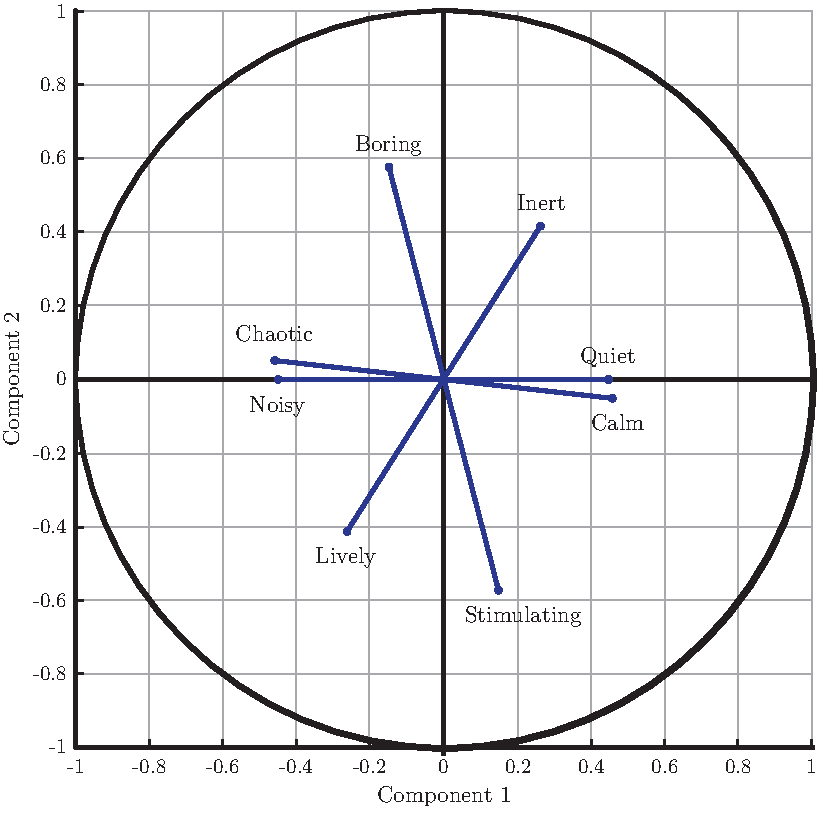
\includegraphics[width=0.8\columnwidth]{pca.pdf}}
  \caption{Principal component analysis (first two components) of the four general perceptual parameters at the scene level (n=9). The observed space is distorted although comparable that of previous works in the literature.}
  \label{fig:pca}
\end{figure}

As discussed in Section~\ref{sec:char} several models have been established to assess pleasantness as a function of global and source-specific parameters. The main objective of this work is to link physical indicators to perceptual source-specific parameters to ultimately predict pleasantness from acoustical data without perceptual assessments. Thus, physical indicators are computed from the audio tracks obtained during scene simulation. To evaluate the overall loudness of the scene, three measurements are chosen in accordance to previous studies~\cite{decoensel2006, ricciardi2014, aumond2017}:
\begin{itemize}
\item $L_{50}$: Z-weighted (no weighting over the observed frequency range) sound level exceeded 50\% of the time in dB,
\item $L_{A50}$: A-weighted sound level exceeded 50\% of the time in dBA,
\item $L_{50}$ for the 1kHz band only.
\end{itemize}


\begin{table*}[ht!]
\centering
\caption{Pearson correlation coefficients between perceptual parameters and physical indicators at the scene level (n=9). *: $p<0.05$, **: $p<0.01$, non-significant correlations ($p>0.05$) are noted NS.}
\label{table:pearsonc}
\resizebox{2\columnwidth}{!}{
\begin{tabular}{ l | c c c c c c c c c c c c c c }
\hline
	Phys./Perc. & OL & I & L & C & $L_{T,p}$ & $T_{T,p}$ & $L_{B,p}$ & $T_{B,p}$ & $L_{H,p}$ & $T_{H,p}$ & $L_{V,p}$ & $T_{V,p}$ & $L_{F,p}$ & $T_{F,p}$ \\ \hline
	$L_{50,1kHz}$ & 0.93** & NS & NS & -0.92** & 0.75* & 0.7* & NS & NS & NS & NS & NS & NS & NS & NS \\
	$L_{50}$ & 0.98** & NS & 0.73* & -0.97** & 0.72* & NS & NS & NS & NS & NS & NS & NS & NS & NS \\
	$L_{A50}$ & 0.96** & NS & 0.73* & -0.94** & NS & NS & NS & NS & NS & NS & NS & NS & NS & NS \\ \hline
	$T_T$ & NS & NS & NS & NS & NS & NS & NS & NS & NS & NS & NS & NS & NS & NS \\
	$L_T$ & NS & NS & NS & NS & NS & NS & NS & NS & NS & NS & NS & NS & NS & NS \\ \hline
	$T_B$ & NS & 0.67* & NS & NS & 0.71* & 0.75* & NS & NS & NS & NS & NS & NS & NS & NS \\
	$L_B$ & NS & 0.93** & NS & NS & -0.84** & -0.83** & 0.91** & 0.82** & NS & NS & NS & NS & NS & NS \\ \hline
	$T_H$ & NS & NS & NS & NS & NS & NS & NS & NS & NS & 0.84** & NS & NS & NS & NS \\
	$L_H$ & NS & NS & NS & NS & NS & NS & NS & NS & 0.98** & 0.78* & NS & NS & NS & NS \\ \hline
	$T_V$ & NS & NS & NS & NS & NS & NS & NS & NS & NS & NS & NS & NS & NS & NS \\
	$L_V$ & NS & NS & 0.81** & NS & NS & NS & NS & NS & NS & NS & 0.84** & 0.88** & NS & NS \\ \hline
	$T_F$ & NS & NS & NS & NS & NS & NS & NS & NS & NS & NS & NS & NS & 0.9** & 0.68* \\
	$L_F$ & NS & NS & -0.72* & NS & NS & NS & NS & NS & NS & NS & -0.69* & -0.78* & 0.92** & NS \\ \hline
	$T_T(\alpha)$ & NS & -0.81** & NS & NS & 0.90** & 0.94** & NS & NS & NS & NS & NS & NS & NS & NS \\
	$T_T(\alpha, \beta)$ & NS & -0.80** & NS & NS & 0.88** & 0.92** & NS & NS & NS & NS & NS & NS & NS & NS \\ \hline
	$T_B(\alpha)$ & NS & 0.88** & NS & NS & NS & NS & 0.95** & 0.97** & NS & NS & NS & NS & NS & NS \\
	$T_B(\alpha, \beta)$ & NS & 0.88** & NS & NS & NS & NS & 0.95** & 0.97** & NS & NS & NS & NS & NS & NS \\ \hline
	$T_H(\alpha)$ & NS & NS & NS & NS & NS & NS & NS & NS & NS & 0.83** & NS & NS & NS & NS \\
	$T_H(\alpha, \beta)$ & NS & NS & NS & NS & NS & NS & NS & NS & 0.73* & 0.88** & NS & NS & NS & NS \\ \hline
	$T_V(\alpha)$ & NS & NS & 0.82** & NS & NS & NS & NS & NS & NS & NS & 0.79* & 0.83** & NS & NS \\
	$T_V(\alpha, \beta)$ & NS & NS & 0.82** & NS & NS & NS & NS & NS & NS & NS & 0.75* & 0.79* & NS & NS \\ \hline
	$T_F(\alpha)$ & NS & NS & NS & NS & NS & NS & NS & NS & NS & NS & NS & -0.71* & 0.87** & NS \\
	$T_F(\alpha, \beta)$ & NS & NS & NS & NS & NS & NS & NS & NS & NS & NS & NS & NS & 0.90** & 0.70* \\ \hline
\end{tabular}
}
\end{table*}

Source-specific indicators are also computed: the time of presence and an emergence estimation metric (resp. $T_s$ and $L_s$ for source $s$), obtained by subtracting the global $L_{90}$ (Z-weighted level exceeded 90\% of the time), found to represent well background activity, to the $L_{10}$ of each source. The emergence is considered for the whole source activity while time of presence can only be associated to sound events. Sound levels are computed with the Matlab ITA toolbox~\cite{itatoolbox2017} in the 20~Hz-20~kHz range.

In the considered scenes, background sources are always active. The measurement of time of presence is thus limited to sound events which leads to relatively poor representation of the ground truth. This is particularly problematic for traffic sources active in the background of most urban soundscapes. Furthermore, the considered indicators are computed for each sound source separately, not taking into account potential masking effects by other sources active at the same time. Two additional indicators are thus designed regarding these considerations.

\subsection{Proposed indicators}


The first proposed indicator $T_s(\alpha)$ is a time of presence metric relying on the emergence of each sound source relative to the others over time. Sound levels (dB) are computed for audio frames of 125~ms. This duration is approximately that of the shortest event found during annotation and corresponds to the "fast" measurements used in acoustical monitoring applications. The emergence, \textit{i.e.} difference $\Delta_s(t)$ of sound levels between the studied source ($L_s(t)$) and the background constituted of all others ($L_b(t)$) is computed. The source is then considered present on a given time frame if the emergence is greater than a threshold value $\alpha$. A time of presence measurement is obtained by averaging over time:
\begin{equation}
T_s(\alpha) = \frac{1}{N_t}\sum_{t = 1}^{N_t}\mathbbm{1}_{\Delta_s(t)>\alpha}
\end{equation}
where $N_t$ is the total number of 125~ms analysis frames in the scene. The optimal threshold is found via grid search to be $\alpha = -31dB$ for the considered corpus. If a source is objectively present it will almost always be considered as present regardless of the other contents of the scene.

However, the masking of a sound by another does not depend only on the emergence over the whole frequency spectrum. The spectral distribution is important, the level comparison shall thus be made around the characteristic frequency components of a source. A second indicator $T_s(\alpha, \beta)$, based on a spectral decomposition is thus proposed. Third-octave bands sound levels are computed on 125\~ms frames and the emergence of a source compared to the background is defined as
\begin{equation}
\Delta_s(t, f) = L_s(t, f) - L_b(t, f)
\end{equation}
Similarly to the first metric $T_s(\alpha, \beta)$ then relies on simple thresholds applied on the emergence, first in frequency then in time. Its expression is as follows:
\begin{equation}
T_s(\alpha, \beta) = \frac{1}{N_t}\sum_{t = 1}^{N_t}\mathbbm{1}\left[ \frac{\sum_{f = 1}^{N_f}\Delta_s(t, f)\mathbbm{1}_{\Delta_s(t, f)>\alpha}}{\sum_{f = 1}^{N_f}\mathbbm{1}_{\Delta_s(t, f)>\alpha}}>\beta \right]
\end{equation}
where $N_f$ is the number of third-octave bands. Here the emergence threshold $\alpha$ is applied to each frequency band of the signal at a given time frame. To determine if the source is heard in the frame a second threshold $\beta$ is then used on the mean emergence of the source on emergent bands. Again, optimal values for parameters $\alpha_{opt} = -6 dB$ and $\beta_{opt} = -5 dB$ are found via grid search on the experiment corpus as no other subset of scenes with both physical and perceptual data is available. This set of values is more plausible physically, as it indicates that a source is considered heard if its sound level is at most 5~dB lower than that of other sources overlapping in time and frequency.

Table~\ref{table:pearsonc} shows the Pearson's correlation coefficients between the computed indicators and assessed parameters at the sound scene level (n=9). The three globally computed sound levels $L_{50}$, $L_{A50}$ and $L_{50,1kHz}$ represent well the perceived overall loudness of the scene and can be used directly for pleasantness prediction. Ground truth emergences also correlate with the evaluated sound level parameters for all sources but traffic. The perceived time of presence is however represented poorly by both ground truth time of presence and emergence metrics: the source time of presence fails to account for potential masking by other sounds and the long-term emergence does not consider time distribution of activity. The two proposed emergence-based time of presence indicators exhibit better behaviors: they are discriminative and show high correlations with the perception of corresponding sources. This confirms the need of an emergence-based presence indicator to successfully represent heard sources in the scene's mix.

For all sources the perceived time of presence and sound level are highly correlated ($r>0.8, p<0.01$). This is not the case for the corresponding acoustical indicators indicating information redundancy between these two quantities at the perceptual level. As a result one of the two quantities is often omitted in proposed pleasantness models.

\section{Conclusion}
\label{sec:disc}

A pilot experiment was performed to assess the relevance of predicting perceptual parameters from acoustic indicators in simulated scenes for soundscape quality assessment. The ground truth time of presence of sources is found not sufficient to fully characterize soundscape perception. Some sources can be active but not heard in the mix, especially background sounds such as continuous traffic. This illustrates the need to account for source emergence as a metric to determine their perceptual importance in complex soundscapes. The proposed indicator $T_s(\alpha, \beta)$, while relying on a simple emergence model due to the small amount of available data, can be directly linked to source-specific perceptual quantities. Predicting the average pleasantness of a soundscape can thus be achieved by estimating the source activity and emergence indicators proposed in Section~\ref{sec:char}.

Precision requirements of the postulated physical metrics are also obtained. The 125~ms or longer time scales used for the computation of all indicators in the presented experiment allow the design of perceptually relevant indicators. A binary (not heard - heard) masking model is shown in this study to improve parameter prediction. The estimation of source-wise emergence as a classification process (4 classes from \textit{Not heard at all} to \textit{Dominant}) as opposed to continuous regression is thus considered sufficient for the application needs.

Future work will 1) consider a refined perceptual experiment with a richer soundscape corpus in order to achieve a stronger validation and model design and 2) formulate a complete experimental protocol dedicated to the soundscape characterization task.

\bibliographystyle{IEEEtran}
\bibliography{refs}

\end{sloppy}
\end{document}
